%||||||||||||||||||||||||||||||||||||||||||||||||||||||||||||||||||
%||||                  READING INSTRUCTIONS                    ||||
%||||||||||||||||||||||||||||||||||||||||||||||||||||||||||||||||||
%||||                                                          ||||
%|||| > Start by looking over the main file                    ||||
%|||| > Then go through the Examples                           ||||
%||||    - It is very important that you have the compiled pdf ||||
%||||    - on the side when reading the code. Rhe information  ||||
%||||    - is closely tied together and equally important.     ||||
%|||| > There are also some notes in the bibliography          ||||
%||||    - Its location: setup/bibliography.bib                ||||
%|||| > In "Chapter 1" you will find a text-example            ||||
%|||| > In "Appendix A" you will find an example of how to     ||||
%||||   make a measurement report. The text concerning the     ||||
%||||   test itself is not important, but is left there to     ||||
%||||   assist in proving a structural example.                ||||
%||||                                                          ||||
%|||| I recomend that you do not read the macro file fist :)   ||||
%||||                                                          ||||
%|||| The comments have been written on a rather large screen, ||||
%|||| if it seems messy try disabling word wrap while reading. ||||
%|||| Remember to switch it back afterwards :)                 ||||
%||||    In TeXstudio:                                         ||||
%||||    Options                                               ||||
%||||    --> Configure Texstudio...                            ||||
%||||    --> Adv. Editor                                       ||||
%||||    --> under Special Options                             ||||
%||||    --> (in the middle) Line Wrapping:                    ||||
%||||    --> choose No Line Wrap                               ||||
%||||                                                          ||||
%||||||||||||||||||||||||||||||||||||||||||||||||||||||||||||||||||
%||||||||||||||||||||||||||||||||||||||||||||||||||||||||||||||||||

%preamble - package unclusion and set up
%page setup (page size, text size, page layout, chapters start on a new page).
%memoir is a form of book class that supports any kind of document.
\documentclass[fleqn,a4paper,12pt,twoside,openany]{memoir}

%setting the header and footer in that order:
\setheadfoot{28pt}{28pt} %if any problems are encountered, try changing the latter 28pt with 1cm.

%general package syntax: \usepackage[options]{package}

%setting language:
\RequirePackage[danish, english]{babel}

\usepackage{siunitx}

%this package makes it possible to treat any element as a float,
%figures and tables are by default treated as floats.
%read http://en.wikibooks.org/wiki/LaTeX/Floats,_Figures_and_Captions to specify your float.
\usepackage{float}
\usepackage{wrapfig}
\usepackage{placeins}

%this package makes it possible to make theorems and examples:
\usepackage{amsthm}
%setting the style of examples (parameters: plain, definition, remark):
%(definition is usually used for examples)
\theoremstyle{definition}
%the frist parameter is the syntax used in the document, the second is that which is printed in LaTex.
\newtheorem{example}{Eksempel}

%making it possible to use æ, ø and å:
\usepackage[utf8]{inputenc}
%helps with word division when using æ, ø and å, and makes it ps-font rather than bmp:
\usepackage[T1]{fontenc}

%package for implementation of graphic files:
\usepackage{graphicx}

%package for captions
\usepackage[nooneline]{caption}

%%package for implementation of math:
\usepackage{amsmath , amsfonts , amssymb, float}

%allowing use of color:
\usepackage{color}
%allowing use of more colors also in tables (see: http://en.wikibooks.org/wiki/LaTeX/Colors):
\usepackage[usenames,dvipsnames,svgnames,table]{xcolor}

%hyperlinks in the tabel of contents - comment this out before the report is printed.
\usepackage{hyperref}
\hypersetup{
	bookmarks = true,  % Show 'bookmark'-frame in pdf.
	colorlinks = true, % True = colored links, False = framed links.
	citecolor = blue,  % Link color for references.
	linkcolor = blue,  % Link color in table of contents.
	urlcolor = blue,   % Link color for extern URLs.
}

%makes it possible to refer to the name of a chapter rather than just the number.
\usepackage{nameref}

%package for writing program code in latex
\usepackage{listings}

\lstset{ 
language=C,               	 	% choose the language of the code
basicstyle=\footnotesize,       % the size of the fonts that are used for the code
numbers=left,                   % where to put the line-numbers
numberstyle=\footnotesize,      % the size of the fonts that are used for the line-numbers
stepnumber=1,                   % the step between two line-numbers. If it is 1 each line will be numbered
numbersep=5pt,                  % how far the line-numbers are from the code
backgroundcolor=\color{white},  % choose the background color. You must add \usepackage{color}
showspaces=false,               % show spaces adding particular underscores
showstringspaces=false,         % underline spaces within strings
showtabs=false,                 % show tabs within strings adding particular underscores
frame=single,           		% adds a frame around the code
tabsize=2,          			% sets default tabsize to 2 spaces
captionpos=b,           		% sets the caption-position to bottom
breaklines=true,       			% sets automatic line breaking
breakatwhitespace=false,    	% sets if automatic breaks should only happen at whitespace
escapeinside={\%*}{*)}          % if you want to add a comment within your code
}

%setting references (using numbers) and supporting i.a. Chicargo-style:
\usepackage{etex}
\usepackage{etoolbox}
\usepackage{keyval}
\usepackage{ifthen}
\usepackage{url}
\usepackage{csquotes}
\usepackage[backend=biber,url=true,doi=true,style=numeric,sorting=none]{biblatex}
\bibliography{myBib.bib}

%this package makes it possible include pdf pages in fx appendix;
%using  following syntax: \includepdf[pages={1}]{myfile.pdf}
\usepackage{pdfpages}

%%%MARGINER%%%
\setlrmarginsandblock{3.5cm}{2.5cm}{*}	% \setlrmarginsandblock{inner margin}{outer margin}{ratio}
\setulmarginsandblock{2.5cm}{3.0cm}{*}	% \setulmarginsandblock{top}{bottom}{ratio}
\checkandfixthelayout 			            % fixes stuff..

%Enables the use FiXme refferences. Syntax: \fixme{...}
%With "final" in stead of "draft" an error will ocure for every FiXme
%under compilation.
\usepackage[footnote,draft,english,silent,nomargin]{fixme}

%%%CHAPTERLAYOUT%%%
%setting the color of the chapter number
\definecolor{numbercolor}{gray}{0.7}
%Downloaded chapter-setup:
\newif\ifchapternonum
\makechapterstyle{jenor}{
  \renewcommand\printchaptername{}
  \renewcommand\printchapternum{}
  \renewcommand\printchapternonum{\chapternonumtrue}
  \renewcommand\chaptitlefont{\fontfamily{pbk}\fontseries{db}\fontshape{n}\fontsize{25}{35}\selectfont\raggedleft}
  \renewcommand\chapnumfont{\fontfamily{pbk}\fontseries{m}\fontshape{n}\fontsize{1in}{0in}\selectfont\color{numbercolor}}
  \renewcommand\printchaptertitle[1]{%
    \noindent
    \ifchapternonum
    \begin{tabularx}{\textwidth}{X}
    {\let\\\newline\chaptitlefont ##1\par} 
    \end{tabularx}
    \par\vskip-2.5mm\hrule
    \else
    \begin{tabularx}{\textwidth}{Xl}
    {\parbox[b]{\linewidth}{\chaptitlefont ##1}} & \raisebox{-15pt}{\chapnumfont \thechapter}
    \end{tabularx}
    \par\vskip2mm\hrule
    \fi
  }
}
%setting chapter style:
\chapterstyle{jenor}

%depth of numbered headlines (part/chapter/section/subsection):
\setsecnumdepth{none}
\maxsecnumdepth{none}
%depth of the table of contents:
\settocdepth{section}

% Makes sure LaTeX does not stretch the text at page break:
\raggedbottom

%macros - please read this file
%%%%%%%%%%%%%%%%%%%%%%%%%%%%%%%%%%%%%%%%%%%%%%%%%%%%%
%             UNITS, EQUATIONS AND TEXT             %
%%%%%%%%%%%%%%%%%%%%%%%%%%%%%%%%%%%%%%%%%%%%%%%%%%%%%
%Units:
\newcommand{\unit}[1]{&& \left[\si{#1}\right]} %\newcommand{\unit}[1]{[\si{#1}]}             <<| Use these if you want equations to be
\newcommand{\unitWh}[1]{[\si{#1}]}             %\newcommand{\eq}[2]{&&\si{#1} &= \si{#2}&&}  <<| centered.. .. will appear scrambled
\newcommand{\numUnit}[1]{\ \si{#1}&}           %                                               | from one equation to the next though..
%Equation:                                     %                                               | and does not work with long equations.. :/
\newcommand{\eq}[2]{\si{#1} &= \si{#2}}
\newcommand{\arw}{&& &\Updownarrow&&}
\newcommand{\eqOne}[2]{\si{#1} &= \si{#2} &\nonumber\\}
\newcommand{\eqTwo}[1]{&\ \ \ \ \si{#1}&}
%Text:
\newcommand{\tx}[1]{\text{#1}}
%Vectors
\renewcommand{\vec}[1]{\boldsymbol{\mathbf{#1}}}
%Vertical line in equations ie. |_x=y (whereTwo stacks two equalities at the line)
\newcommand{\where}[1]{ \left.\rule{0cm}{.5cm}\right\vert\rule{0cm}{.4cm}_{\substack{\rule{0cm}{.15cm}\\ \si{#1} }} }
\newcommand{\whereTwo}[2]{ \left.\rule{0cm}{.67cm}\right\vert\rule{0cm}{.5cm}_{\substack{\si{#1} \rule{0cm}{.19cm}\\\vspace{-.1cm}\\ \si{#2}}} }

%%%%%%%%%%%%%%%%%%%%%%%%%%%%%%%%%%%%%%%%%%%%%%%%%%%%%
%                 TIKZ SETTINGS                     %
%%%%%%%%%%%%%%%%%%%%%%%%%%%%%%%%%%%%%%%%%%%%%%%%%%%%%
\tikzset{
  block/.style    = {draw, thick, rectangle,
                     minimum height = 3em,
                     minimum width = 3em},
  sum/.style      = {draw, circle}, % Adder
}

%%%%%%%%%%%%%%%%%%%%%%%%%%%%%%%%%%%%%%%%%%%%%%%%%%%%%
%                  REFERENCES                       %
%%%%%%%%%%%%%%%%%%%%%%%%%%%%%%%%%%%%%%%%%%%%%%%%%%%%%

%Chapter
\newcommand{\Chapref}[1]{\emph{Chapter \ref{#1}}}
\newcommand{\chapref}[1]{\emph{chapter \ref{#1}}}
%Section
\newcommand{\Secref}[1]{\emph{Section \ref{#1}}}
\newcommand{\secref}[1]{\emph{section \ref{#1}}}
%subSection
\newcommand{\Subsecref}[1]{\emph{Subsection \ref{#1}}}
\newcommand{\subsecref}[1]{\emph{subsection \ref{#1}}}
%Appendix
\newcommand{\Appref}[1]{\emph{Appendix \ref{#1}}}
\newcommand{\appref}[1]{\emph{appendix \ref{#1}}}
%Listings
\newcommand{\Coderef}[1]{\emph{Listings: \ref{#1}}}
\newcommand{\coderef}[1]{\emph{listings: \ref{#1}}}
%Figure:
\newcommand{\Figref}[1]{\emph{Figure \ref{#1}}}
\newcommand{\figref}[1]{\emph{figure \ref{#1}}}
%Table:
\newcommand{\Tableref}[1]{\emph{Table \ref{#1}}}
\newcommand{\tableref}[1]{\emph{table \ref{#1}}}

%Expressions:
\newcommand{\Expr}[1]{\emph{Expression (\ref{#1})}}
\newcommand{\expr}[1]{\emph{expression (\ref{#1})}}

%Equations:
%1 equation:
\newcommand{\Eqref}[1]{\emph{Equation (\ref{#1})}}
\renewcommand{\eqref}[1]{\emph{equation (\ref{#1})}}
%2 equations:
\newcommand{\EqrefTwo}[2]{\emph{Equation (\ref{#1})} and \emph{(\ref{#2})}}
\newcommand{\eqrefTwo}[2]{\emph{equation (\ref{#1})} and \emph{(\ref{#2})}}
%3 equations:
\newcommand{\EqrefThree}[3]{\emph{Equation (\ref{#1})}, \emph{(\ref{#2})} and \emph{(\ref{#3})}}
\newcommand{\eqrefThree}[3]{\emph{equation (\ref{#1})}, \emph{(\ref{#2})} and \emph{(\ref{#3})}}
%4 equations:
\newcommand{\EqrefFour}[4]{\emph{Equation (\ref{#1})}, \emph{(\ref{#2})}, \emph{(\ref{#3})} and \emph{(\ref{#4})}}
\newcommand{\eqrefFour}[4]{\emph{equation (\ref{#1})}, \emph{(\ref{#2})}, \emph{(\ref{#3})} and \emph{(\ref{#4})}}
%5 equations:
\newcommand{\EqrefFive}[5]{\emph{Equation (\ref{#1})}, \emph{(\ref{#2})}, \emph{(\ref{#3})}, \emph{(\ref{#4})} and \emph{(\ref{#5})}}
\newcommand{\eqrefFive}[5]{\emph{equation (\ref{#1})}, \emph{(\ref{#2})}, \emph{(\ref{#3})}, \emph{(\ref{#4})} and \emph{(\ref{#5})}}
%6 equations:
\newcommand{\EqrefSix}[6]{\emph{Equation (\ref{#1})}, \emph{(\ref{#2})}, \emph{(\ref{#3})}, \emph{(\ref{#4})}, \emph{(\ref{#5})} and \emph{(\ref{#6})}}
\newcommand{\eqrefSix}[6]{\emph{equation (\ref{#1})}, \emph{(\ref{#2})}, \emph{(\ref{#3})}, \emph{(\ref{#4})}, \emph{(\ref{#5})} and \emph{(\ref{#6})}}
%7 equations:
\newcommand{\EqrefSeven}[7]{\emph{Equation (\ref{#1})}, \emph{(\ref{#2})}, \emph{(\ref{#3})}, \emph{(\ref{#4})}, \emph{(\ref{#5})}, \emph{(\ref{#6})} and \emph{(\ref{#7})}}
\newcommand{\eqrefSeven}[7]{\emph{equation (\ref{#1})}, \emph{(\ref{#2})}, \emph{(\ref{#3})}, \emph{(\ref{#4})}, \emph{(\ref{#5})}, \emph{(\ref{#6})} and \emph{(\ref{#7})}} %TIP: If you are using TeXstudio you can open
                         %     the file by Ctrl+LeftClick on setup/macros.tex
\begin{document}         %     If the file doesn't exist, you will be asked
\tableofcontents         %     weather or not you want to create it.
\pagebreak

%||||||||||||||||||||||||||||||||||||||||||||||||||||||||||||||||
%|||||||     Intended use of Template during Project     ||||||||
%||||||||||||||||||||||||||||||||||||||||||||||||||||||||||||||||
%||||                                                        ||||
%|||| In the beginning it seems silly not to just work       ||||
%|||| directly in the main file, however, as the project     ||||
%|||| grows it takes more and more time to compile, so       ||||
%|||| it might be preferable to compile with a template      ||||
%|||| like this.                                             ||||
%|||| You can uncomment everything else than the section     ||||
%|||| you are currently working on, without doing any        ||||
%|||| damage when you forget to comment the                  ||||
%|||| section back in :)                                     ||||
%|||| The intention is also for the template to be used      ||||
%|||| as a resource when in doubt of conventions or syntax.  ||||
%||||                                                        ||||
%||||||||||||||||||||||||||||||||||||||||||||||||||||||||||||||||
%||||||||||||||||||||||||||||||||||||||||||||||||||||||||||||||||


%||||||||||||||||||||||||||||||||||||||||||||||||||||||||||||||||
%|||||||                 Example Inputs                  ||||||||
%||||||||||||||||||||||||||||||||||||||||||||||||||||||||||||||||
%|||||||                                                 ||||||||
           \chapter{Figure Sample}

%IMPORTANT NOTE%
%Put the editable image source file (if this exists) in the Source folder!

                                                    % The fxnote is the reason that the caption
                                                    % is left aligned instead of centered.
                                                    % Furthermore, it does not show the fxnote in
\begin{figure}[H]                                   % a footnote.
  \centering                                        % It does however appear in list of corrections.
  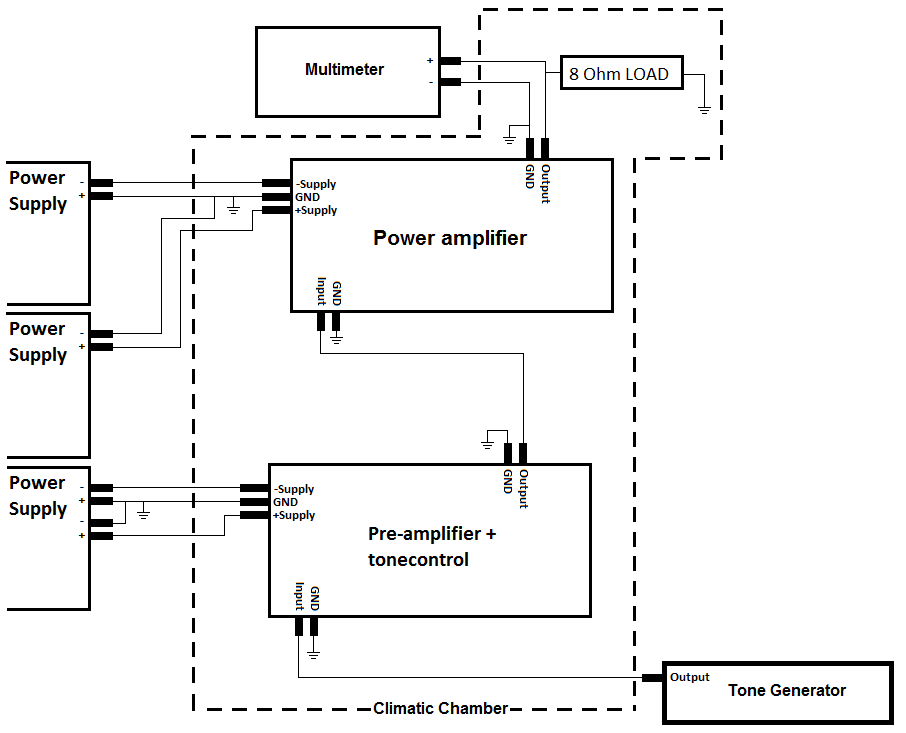
\includegraphics[scale=.3]{figures/filename}
  \caption{This image is clearly too small, remember to scale appropriately\fxnote{Remember source}}
  \label{FigureLABEL}     %<--give the figure a lable, so you can reference!
\end{figure}              %   For the label to work it must be under the caption.

%--------- NOTES ------------------------------------------------------
%Fxnotes wont compile properly inside the figure, only in the caption.
%File-type ([...]{figures/filename.jpg}) can be specified but isn't needed.
%
\Figref{FigureLABEL} $\leftarrow$ this is used in the beginning of a sentence, whereas \figref{HbridgeClokwise4Q} is used in the middle of a sentence\fxnote{This however does work in the footnote}.

%Do not use \vspace{length}, \hspace{length} or \noindent etc. unless exceedingly necessary - LaTeX is a markup language, let it do its job.
\vspace{.5cm}
\noindent
%--------- BIBLIOGRAPHY REF EKSAMPLE -----------------------------------
This reference only represents this line since it is before the punctuation mark\cite{YDing}. This next reference however represents the entire section. That is, all of the preceding sentences in the entire section. This is due to the fact that it is now after the punctuation mark in the end of the section (this is not used in the middle of a section!).\cite{YDing}
%>>>>>>>>>>>>>>>PLEASE ALSO READ THE NOTE IN bibliography/bibliography.bib<<<<<<<<<<<<<<<<<<

Here is a \st{good} messy way to make two images appear on the side of each other. Also, if you modified an image, this is how you properly refer to its original source:

  \begin{minipage}{\linewidth}
  	\begin{minipage}{0.45\linewidth}
  		\begin{figure}[H]
  			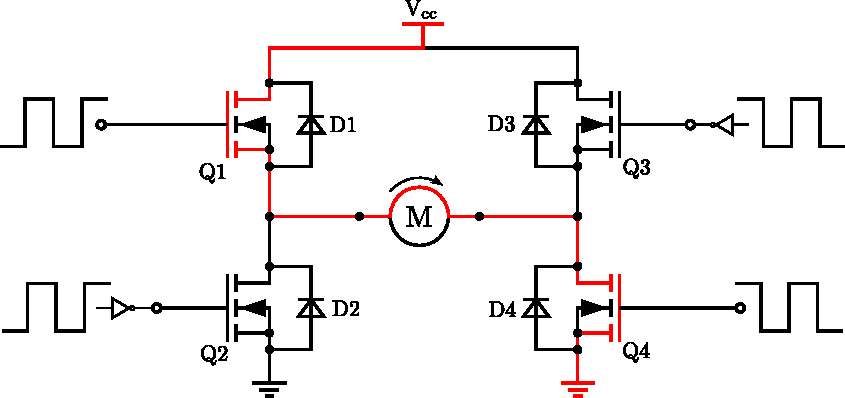
\includegraphics[scale=.53]{figures/HbridgeClockwise4Q.pdf}
  			\centering
  			\vspace{-.4cm}
  			\captionsetup{justification=centering}
  			\captionof{figure}{Clockwise 4Q operation.\\ \emph{Edited from image by Biezl}.\cite{Biezl}}
  			\label{HbridgeClokwise4Q}
  		\end{figure}\vspace{-5mm}
  	\end{minipage}
  	\hspace{0.03\linewidth}
  	\begin{minipage}{0.45\linewidth}
  		\begin{figure}[H]
  			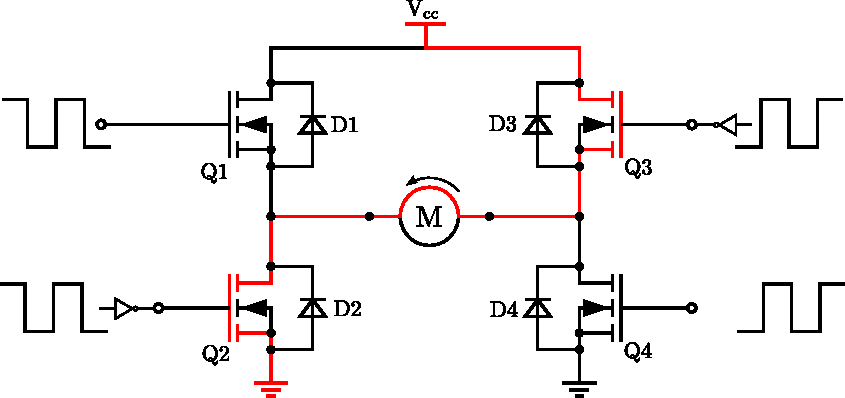
\includegraphics[scale=.53]{figures/HbridgeCounterClockwise4Q.pdf}
  			\centering
  			\vspace{-.4cm}
  			\captionsetup{justification=centering}
  			\captionof{figure}{Counterclockwise 4Q operation.\\ \emph{Edited from image by Biezl}.\cite{Biezl}}
  			\label{HbridgeCounterClokwise4Q}
  		\end{figure}\vspace{-5mm}
  	\end{minipage}
  \end{minipage}

\pagebreak           %|||||||
           \section{Table Sample}

\begin{table}[H]
\begin{tabular}{|l|p{5cm}|l|l|l|}
  \hline %-----------------------------------------------------------------------------------
  \textbf{No.} &\textbf{Description} &\textbf{Min} &\textbf{Max} &\textbf{Requirements}    \\
  \hline %-----------------------------------------------------------------------------------
  1            & Some Text           & Some Text   & Some Text   & Some Text               \\
               &                     &             &             & Some More Text          \\
               &                     &             &             & Text Text               \\
               &                     &             &             & Text Text Text          \\
  \hline %-----------------------------------------------------------------------------------
  2            & Some Text           & Some Text   & Some Text   & Some Text               \\
  \hline %-----------------------------------------------------------------------------------
  3            & By specifying the
                 width of a column
                 (|p\{5cm\}|) the
                 cells in that column
                 will not exceed the
                 specified width but         %Extra whitespace is used only for clarity
                 instead expand              %and will not affect the compiled output.
                 downward.
                                     & Some Text           & Some Text   & Some Text       \\
  \hline %-----------------------------------------------------------------------------------
  4            & Some Text           & Some Text   & Some Text   & Some Text               \\
  \hline %-----------------------------------------------------------------------------------
  \multicolumn{2}{|l|}{Some Text}    & \multicolumn{3}{l|}{Some Text}                      \\
  \hline %-----------------------------------------------------------------------------------
  \multicolumn{2}{|l|}{Text Text}    & \multicolumn{3}{l|}{Text = Text}                    \\
  \multicolumn{2}{|l|}{}             & \multicolumn{3}{l|}{Text = Text}                    \\
  \multicolumn{2}{|l|}{}             & \multicolumn{3}{l|}{Text = Text}                    \\
  \multicolumn{2}{|l|}{}             & \multicolumn{3}{l|}{Text = Text}                    \\
  \multicolumn{2}{|l|}{}             & \multicolumn{3}{l|}{Text = Text}                    \\
  \hline %-----------------------------------------------------------------------------------
  \multicolumn{2}{|l|}{Some Text}    & \multicolumn{3}{l|}{Teeeexxtt}                      \\
  \multicolumn{2}{|l|}{}             & \multicolumn{3}{l|}{\LaTeX}                         \\
  \hline %-----------------------------------------------------------------------------------
\end{tabular}
\caption{This Is a Table\label{TableLABEL}}
\end{table}

\Tableref{TableLABEL} $\leftarrow$ this is used in the beginning of a sentence, whereas \tableref{TableLABEL} is used in the middle of a sentence.

\pagebreak            %|||||||
           \section{Equation Sample} %<-- IMPORTANT! In American English all Important Words in Headlines are with Big Letters

%\eq is a macro, which even includes the equal-sign - this has been done, so that, if we wish to change
%the appearance of equations, this can easily be done from the macro. Please use it :)

%\unit is an other macro. It uses SI units and aligns all the units neatly :)
%   SI is written with negative exponents rather than using fraction bars, that is:
%   rad \cdot s^{-2} rather than \frac{ rad }{ s^{2} }
%Note that \unit is used in the equation, and \unitWh is used in the "Where:"-statements,
%This is due to a macro workaround - see the macro file for more information on this.

%I know I said never to write something like: \hspace{6mm} Where:\\, this is the exception from the rule :)

\textbf{A normal equation:}
\begin{flalign}
  \eq{J_m \cdot \dot{\omega}_m(t)} {\tau_m(t) - B_m \cdot \omega_m(t) - r_m \cdot f_c(t)}\unit{N \cdot m} 
  \label{MotorGearNewtonSecLaw}
\end{flalign}
%
\hspace{6mm} Where:\\
\begin{tabular}{ p{1cm} l l l}
& $J_m$ 					    	& is the motor's inertia                        &\unitWh{kg \cdot m^2} \\
& $\omega_m(t)$         & is the angular velocity of the motor          &\unitWh{rad \cdot s^{-1}} \\
& $\dot{\omega}_m(t)$ 	& is the angular acceleration of the motor      &\unitWh{rad \cdot s^{-2}} \\
& $\tau_m(t)$ 			    & is the torque delivered by the motor          &\unitWh{N \cdot m} \\
& $B_m$                 & is the motor's friction coefficient           &\unitWh{N \cdot m \cdot s \cdot rad^{-1}} \\
& $r_m$                 & is the radius of the gear, $G_m$              &\unitWh{m} \\
& $f_c(t)$							& is the contact force between the two gears    &\unitWh{N}
\end{tabular}

\textbf{If you need to write some expression without an equal sign:}
\begin{flalign} 
  &\si{ \frac{r_m\cdot r_t}{r_d} \cdot M + \frac{r_d}{2\cdot \pi \cdot r_m \cdot r_t} \cdot J_m + \frac{r_m}{2\cdot \pi \cdot r_t \cdot r_d} \cdot J_d }\label{JTotLinear}&
\end{flalign} 

\Expr{JTotLinear} is referencing to \expr{JTotLinear}, but in the beginning of a sentence.

\textbf{If you need to write something with numbers:}
\begin{flalign}
  \eq{B}{\num{2,2}\cdot 10^{-6}} \ \si{N\cdot m \cdot rad^{-1} \cdot s}& \label{eq2} \\ %<-- if you want two equations to
  \eq{\tau_c}{\num{0.0016}}      \ \si{N\cdot m}                       & \label{eq3}    %    allign in one envirenment,
\end{flalign}                                                                           %    remember \\

\textbf{To reference several equations in a sentence:}\\ %<-- Usually it is best to use subsubsections rather than \textbf{}
%                                                             However!
\eqrefTwo{MotorGearNewtonSecLaw}{eq2}\\                  %    You do not have a subsubsection without also having:
%                                                        %    A subsection, a section and a chapter above it.
\eqrefThree{MotorGearNewtonSecLaw}{eq2}{eq3}\\

\textbf{To reference several equations in the beginning of a sentence:}\\
%
\EqrefTwo{MotorGearNewtonSecLaw}{eq2}\\
%
\EqrefThree{MotorGearNewtonSecLaw}{eq2}{eq3}\\

\textbf{This works for up to 7 equations.}

\pagebreak         %|||||||
           \begin{figure}[H]
  \begin{tikzpicture}[ auto,
                       thick,                         %<--setting line style
                       node distance=2cm,             %<--setting default node distance
                       scale=1.5,                     %<--|these two scale the whole thing
                       every node/.style={scale=1.5}, %<  |(always change both)
                       >=triangle 45 ]                %<--sets the arrowtype
    \draw%--------------------------------------------------------------------------------------------
    	%Drawing the Equation Blocks:
    	
    	%Naming the coordinate (0,0) input1, for later use:
    	node[shape=coordinate][](input1) at (0,0){}
  	
    	%node(sum1)                       ...creates a node with name sum1
    	%[sum, right of = input1]         ...create a sum-circle (defined in macros)
    	%                                    to the right of the input node
    	%{$\sum$}                         ...writes a summation symbol inside the circle
    	node(sum1) [sum, right of = input1] {$\sum$}
  	
    	%at (4.5,0) [block]               ...creates block (as defined in macros) at (4.5,0)
    	%{ $[...]$ }                      ...writes a transfer function in the block
    	node(transferfunction) at (4.8,0) [block] {\Large $\ \frac{a\cdot s + b}{c \cdot s^2 + d \cdot s + e}\ $ }
    
      %node(integrate) at (6.8,0)       ...creates a node with name integrate @ (6.8,0)
      %[block]                          ...creates a block (as defined in macros) @ specified node
      %{\Large $\frac{1}{s}$}           ...writes an integrator in the block
      node(integrate) at (7.8,0) [block] {\Large $\frac{1}{s}$}
    
      %node(feedBack)                  ...creates node named feedBack
      %[block, below of = block1]      ...creates block below block1
      %{\Large$H(s)$}                  ...writes H(s) in the feed back block
      node(feedBack) [block, below of = transferfunction] {\large$H(s)$}
      
    ;%------------------------------------------------------------------------------------------------
    
    %Joining the Blocks
    %When using \draw with options like [->], each line must be enclosed as follows:
    %\draw[..arrow/line..]  ..handelingOfArrow/Line..  ;
    
    %Naming the coordinate (9,0) output1:
    \draw
      node[shape=coordinate][](output1) at (9,0){}
    ;
    
    % \draw[->](input1) --            ...draws a straight arrow from node with name: input1
    % node {$X(Z)$}(sum1)             ...to the node with name: sum1 .. writes on arrow: X(s)
  	\draw[->](input1) -- node {$X(s)$}(sum1);
  	
  	%same logic for the following as for the previous line
    \draw[->](sum1) -- node {} (transferfunction);
  	\draw[->](transferfunction) -- node {} (integrate);
  	
  	%\draw[->](feedBack)            ...draws an arrow from feedBack block
  	%-| node{} (sum1)               ...makes a 90 degree turn and terminates @ node: sum1
  	\draw[->](feedBack) -| node{} (sum1);

  	%\draw[->] (integrate)          ...draws straight arrow from integrate
  	%-- (output1)                   ...to (output1)
  	%|-                             ...making a 90 degree turn @ (output1)
  	%(feedBack)                     ...connects the arrow from (output1) to node: feedback
  	\draw[-] (integrate) -- (output1);
  	\draw[->] (output1) |- (feedBack);
  	
  	%Drawing output arrow from (output1) to (10.5,0)
  	\draw[->](output1) -- node {$Y(s)$} (10.5,0);

    %Drawing node(s) with \textbullet
    %[shift={... adjusts the position of the bullets
    \draw%--------------------------------------------------------------
      node at (input1)  [shift={(-0.04, -0.05 )}] {\Large \textopenbullet}
    	node at (output1) [shift={( 0.01, -0.03 )}] {\textbullet}
    ;%------------------------------------------------------------------

    %Drawing + and - @ sum-block
    \draw%--------------------------------------------------------------
      node at (sum1) [right = -6.5mm, below = .6mm] {$+$} %<--Plus
      node at (sum1) [right = -3mm, below = 3.9mm]  {$-$} %<--Minus
    ;%------------------------------------------------------------------

  \end{tikzpicture}
  \caption{Some tikzpicture drawing}
\end{figure} %|||||||
%|||||||                                                 ||||||||
%||||||||||||||||||||||||||||||||||||||||||||||||||||||||||||||||
%||||||||||||||||||||||||||||||||||||||||||||||||||||||||||||||||

%---------- Chapter 1 ---------------------------------------- Introduction
\chapter{Chapter 2}
\textbf{Here is the header, usually it is written or at least reviewed after the chapter (or large section) is done, this gives the best result.}\\
\lipsum[8]
\section{Section 2.1} %<-- Only Chapters and sections have numbers, to keep down the number of entries in table of contents
\lipsum[2]
\textbf{TIP: Ctrl+LeftClick in the compiled pdf will let you jump to that particular point in the code. It also works from the code to the pdf.}
\subsection{Subsection 2.1.1}
\lipsum[5]
\subsubsection{Subsubsection 2.1.1.1}
\textbf{As mentioned, do not use a subsubsection without a chapter section and subsection above it - do also avoid using} \verb|\textbf{}| \textbf{for headlines.}\\

%---------- Appendix A ---------------------------------------- Test Title
\chapter{Test} \label{test} %<-- remember to label your test so you can
\textbf{Name: Group 630}\\  %    reference in the appropriate section
\textbf{Date: 21/02 - 2016}

\subsubsection{Purpose}
The purpose of the test.

\subsubsection{Setup}
\begin{figure}[H]
  \centering
	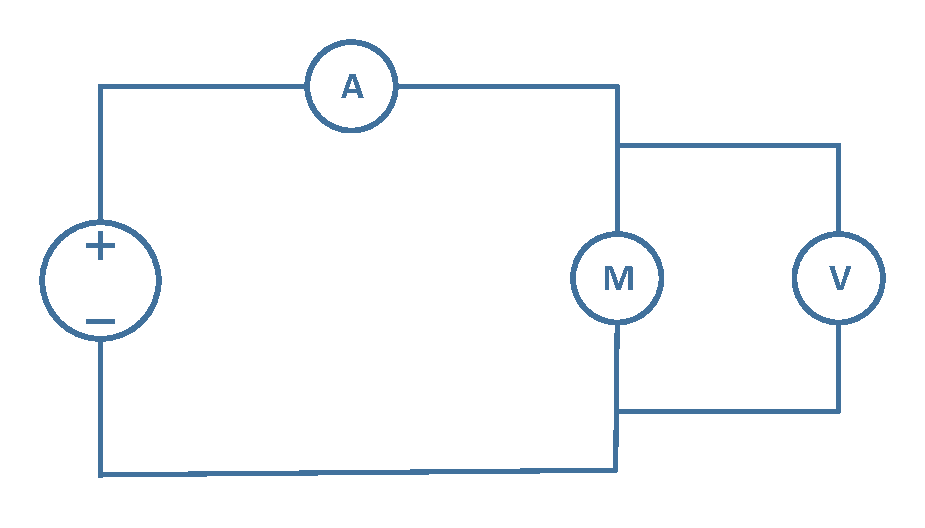
\includegraphics[scale=.45]{figures/MotorTest1.pdf}  %<-- These should be made in something
	\caption{Setup diagram}                              %    else than what this was made in
\end{figure}\vspace{-5mm}                              %    possibly CircuitTikZ for small
                                                       %    conceptual circuits like this.
\subsubsection{List of Equipment}
\begin{table}[H]
\begin{tabular}{|l|l|p{4cm}|}
\hline%------------------------------------------------------------------------------------
  \textbf{Instrument}                        &  \textbf{AAU-no.}  &  \textbf{Type}       \\
\hline%------------------------------------------------------------------------------------
  Multimeter 1                               &  60764             &  Fluke 189 True RMS  \\
\hline%------------------------------------------------------------------------------------
  Multimeter 2                   		         &  60769             &  Fluke 189 True RMS  \\
\hline%------------------------------------------------------------------------------------
  Power Supply \small{(0 - 32 V) (0 - 10 A)} &  77076             &  Ea - ps 7032 - 100  \\
\hline%------------------------------------------------------------------------------------
  Clamp for fixing the motor                 &  03039             &                      \\
\hline%------------------------------------------------------------------------------------
\end{tabular}
\end{table}

\subsubsection{Procedure}

\begin{enumerate}
  \item Turn on the two multimeters and choose Voltage and Ampere settings respectively.
  \item Fix the motor shaft so it can not turn.
  \item Choose the first current value (\SI{0,}{A}) on the current limiting of the power supply.
  \item Turn on the power supply and adjust the current limiting in accordance with the ampere meter.
  \item Read the voltage supplied to the motor from the volt meter.
  \item Repeat the three previous steps for each measurement in \SI{0,5}{A} increments up to 5 A.
  \item Switch the poles of the power supply and repeat the measurements in the negative direction.
\end{enumerate}

\subsubsection{Results}

\begin{table}[H]
\centering
\begin{tabular}{|l|l|l| l|l|}
\cline{1-2}\cline{4-5}%-----------------------             ----------------------------------------------
  \textbf{Input (A)}   & \textbf{Output (V)} &\phantom{hey}& \textbf{Input (A)}   & \textbf{Output (V)}\\
\cline{1-2}\cline{4-5}%-----------------------             ----------------------------------------------
  \SI{-5,0}{}          &       \SI{-0,71}{}  &             & \SI{0,5}{}           & \SI{0,16}{}        \\
\cline{1-2}\cline{4-5}%-----------------------             ----------------------------------------------
  \SI{-4,5}{}          &       \SI{-0,65}{}  &             & \SI{1,0}{}           & \SI{0,34}{}        \\
\cline{1-2}\cline{4-5}%-----------------------             ----------------------------------------------
  \SI{-4,0}{}          &       \SI{-0,59}{}  &             & \SI{1,5}{}           & \SI{0,53}{}        \\
\cline{1-2}\cline{4-5}%-----------------------             ----------------------------------------------
  \SI{-3,5}{}          &       \SI{-0,54}{}  &             & \SI{2,0}{}           & \SI{0,62}{}        \\
\cline{1-2}\cline{4-5}%-----------------------             ----------------------------------------------
  \SI{-3,0}{}          &       \SI{-0,43}{}  &             & \SI{2,5}{}           & \SI{0,64}{}        \\
\cline{1-2}\cline{4-5}%-----------------------             ----------------------------------------------
  \SI{-2,5}{}          &       \SI{-0,36}{}  &             & \SI{3,0}{}           & \SI{0,75}{}        \\
\cline{1-2}\cline{4-5}%-----------------------             ----------------------------------------------
  \SI{-2,0}{}          &       \SI{-0,27}{}  &             & \SI{3,5}{}           & \SI{0,78}{}        \\
\cline{1-2}\cline{4-5}%-----------------------             ----------------------------------------------
  \SI{-1,5}{}          &       \SI{-0,20}{}  &             & \SI{4,0}{}           & \SI{0,80}{}        \\
\cline{1-2}\cline{4-5}%-----------------------             ----------------------------------------------
  \SI{-1,0}{}          &       \SI{-0,14}{}  &             & \SI{4.5}{}           & \SI{0.83}{}        \\
\cline{1-2}\cline{4-5}%-----------------------             ----------------------------------------------
  \SI{-0,5}{}          &       \SI{-0,07}{}  &             & \SI{5.0}{}           & \SI{0.88}{}        \\
\cline{1-2}\cline{4-5}%-----------------------             ----------------------------------------------
\end{tabular}                                              %As you can see right above here, if you use
\end{table}                                                %\SI{}{} for numbers, it will replace '.' with ','
                                                           %because ',' is the SI standard.

\textbf{There are sometimes discussions about where to put the following. Sometimes it makes more sense to have it in the section where the test is used. Whichever way is chosen, should be consistent throughout the report.}

\begin{figure}[H]
  \centering
 	%Trim margins @:   left        bottom       right       top                 %  <--|If you feel like cropping a
 	\adjustbox{ trim = {.15\width} {.30\height} {.15\width} {.30\height}, clip }%  <--|pdf-file directly in latex :)
  {
    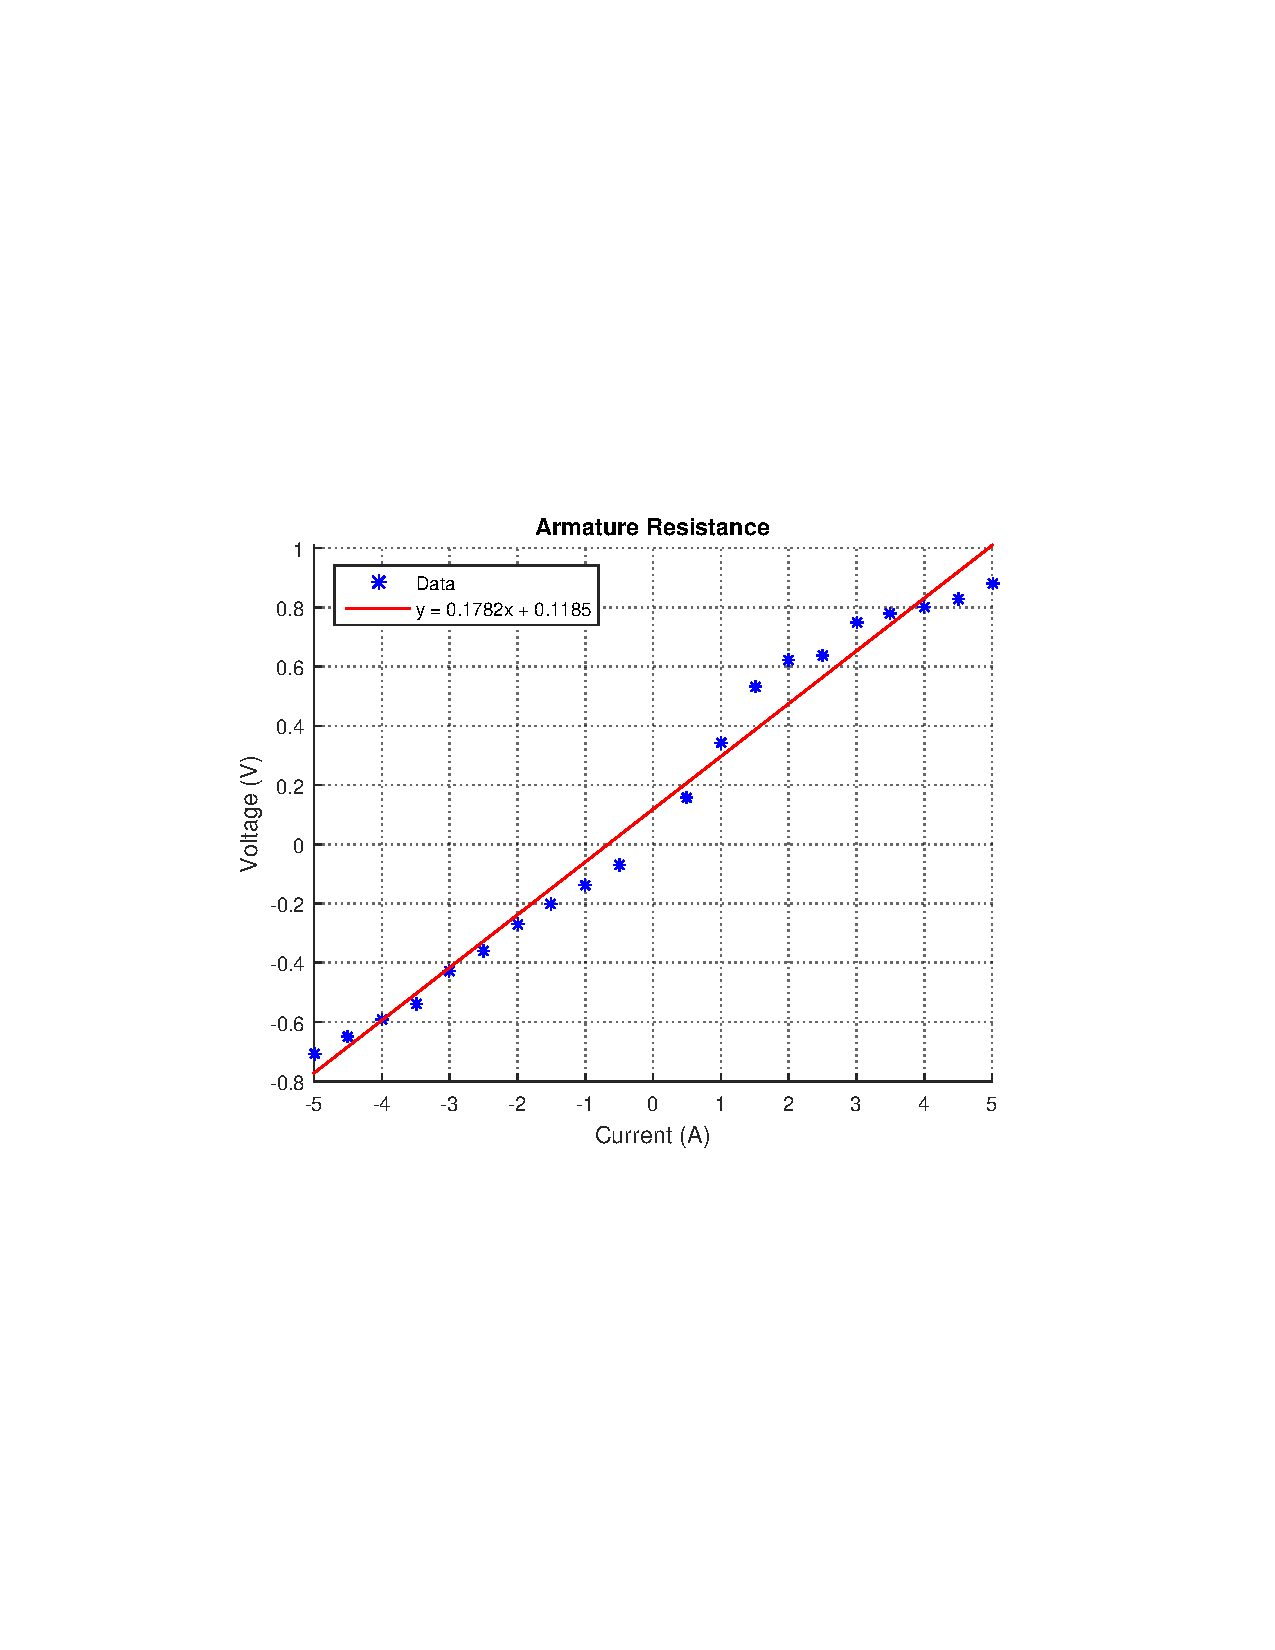
\includegraphics[width=\textwidth]{figures/armatureResistance.pdf}
  }
  \caption{A plot of a measured armature resistance, with a red line indicating the average value.}
  \label{armatureResistance}
\end{figure}

During these measurements the motor is in steady state. This is necessary for the inductor in the armature coil to act as a short circuit, which ease the calculation of the armature resistance. In steady state we get:

\begin{flalign}
  \eq{R_a} {\frac{U_a}{I_a}} \unit{\Omega}
\end{flalign}
\hspace{6mm} Where:\\
\begin{tabular}{p{1cm}lll}
  & \si{I_a} & is the armature current    &\unitWh{A}    \\
  & \si{U_a} & is the armature voltage    &\unitWh{V}    \\
  & \si{R_a} & is the armature resistance &\unitWh{\Omega}  \\
\end{tabular}

As seen on the data plot in \figref{armatureResistance} the result is a relatively linear function. The armature resistance is approximated directly as the slope of the least square line:
\begin{flalign}
  \eq{R_a}{\SI{0,178}{\Omega}}&
\end{flalign}

%%% Bibliography %%%
\printbibliography

%%% List of Corrections
\listoffixmes

\end{document}
